\documentclass[10pt,hyperref={pdfpagemode=FullScreen},aspectratio=169]{beamer}

\usetheme[progressbar=frametitle]{metropolis}
\usepackage{appendixnumberbeamer}
\usepackage{lipsum}
\usepackage{amsmath}
\usepackage{amssymb}
\usepackage{booktabs}
\usepackage{siunitx}
\usepackage[scale=2]{ccicons}
\usepackage{pgfplots}
\usepgfplotslibrary{dateplot}
\usepackage{tikz}
\usetikzlibrary{positioning, shapes.geometric}
\pgfplotsset{compat=newest} % Allows to place the legend below plot
\usepgfplotslibrary{units} % Allows to enter the units nicely
\usepackage{circuitikz}
\usetikzlibrary{shapes,arrows}
\usepackage{dirtytalk}
\usepackage{xspace}




% Bibliography
\usepackage[
    backend=biber,
    style=ieee,
    natbib=true,
    url=false, 
    doi=true,
    eprint=false
]{biblatex}
%\addbibresource{references.bib}


\newcommand{\themename}{\textbf{\textsc{metropolis}}\xspace}
\newcommand{\universidade}{Universidade de Brasília}
\newcommand{\doctitle}{Introduction to AASP}

\definecolor{mpigreen}{HTML}{007977}
\setbeamercolor{frametitle}{bg=mpigreen}

\title{\doctitle}

\author{Daniel Araújo}
\institute{\universidade}
\titlegraphic{\hfill
\includegraphics[height=1.5cm]{../logo}}

\title{Modulação AM}

\author{Prof. Daniel Costa Araújo}

\usepackage{graphicx}
\usepackage{subfigure}
\usepackage{verbatim}
\begin{document}


\frame{\titlepage}


\section{Introdução}

\begin{frame}{O que é modulação?}
  \begin{itemize}
      \item A modulação é o processo de variação de um ou mais parâmetros de uma onda portadora em função do sinal de informação.
      \item Parâmetros comuns a serem modulados:
      \begin{itemize}
          \item Amplitude
          \item Frequência
          \item Fase
      \end{itemize}
      \item A modulação permite transmitir informações a longas distâncias e alocar vários sinais no espectro eletromagnético.
  \end{itemize}
  \end{frame}

\begin{frame}
 
    \frametitle{Conceito}

\begin{block}{Vantagens}

    \begin{itemize}
        \item Conversão de frequência
        \item Redução do tamanho das antenas
        \item Acomodar diferentes sinais 
    \end{itemize}
    
\end{block}


\begin{block}{Tipos de Modulação}
    \begin{itemize}
        \item Double side-band supressed carrier (DSB-SC)
        \item DSB full carrier (DSB-FC)
        \item Single Side Band (SSB)
        \item Vestigial Side Band (VSB)
    \end{itemize}
    
\end{block}
\end{frame}

\section{DSB-SC}

\begin{frame}
    \frametitle{Mensagem} 

    \begin{block}{Definição}
        É a informação que será transmitida pelo canal de comunicação \\        
    \end{block}
    \begin{block}{Exemplo}
        $$ 
        m(t) = A_m cos(2\pi f_m t)
        $$
    \end{block}
    \begin{figure}[!h]
        
\includegraphics[width=0.7\textwidth]{Fig/th-1488438850.jpg}
    \end{figure}
\end{frame}


\begin{frame}
    \frametitle{Exemplo de sinal de Mensagem}

    \begin{figure}[h!]
        \begin{center}
          \begin{tikzpicture}
            \begin{axis}[
                width=0.6\textwidth, % Scale the plot to \linewidth
                grid=major, % Display a grid
                grid style={dashed,gray!30}, % Set the style
                xlabel= Tempo, % Set the labels
                ylabel= Amplitude,
                x unit=\si{\second}, % Set the respective units
                y unit=\si{\volt},
                legend style={at={(1,1)},anchor=north west}, % Put the legend below the plot
                x tick label style={rotate=90,anchor=east} % Display labels sideways
              ]
              \addplot+ [no marks]
              % add a plot from table; you select the columns by using the actual name in
              % the .csv file (on top)
              table[x=Tempo,y=Amplitude(V),col sep=comma] {Fig/sinal_mensagem.csv}; 
              \legend{Sinal mensagem.}
            \end{axis}
          \end{tikzpicture}
          \caption{Sinal mensagem.}
        \end{center}
      \end{figure}
    
\end{frame}


\begin{frame}
    \frametitle{Definição de Portadora}
\begin{itemize}
    \item  Para transmitir a informação, considere um função senoidal  
      
  $$ 
  c(t) = A_c cos(2\pi f_c t + \phi _c)
  $$
    
  \item O sinal modulado na saída do modulador AM-DSB é  

  $$
     s(t) = m(t)*c(t)
  $$

\end{itemize}

\end{frame}

\begin{frame}
    \frametitle{Exemplo de sinal modulado}

    \begin{figure}[h!]
        \begin{center}
          \begin{tikzpicture}
            \begin{axis}[
                width=0.6\textwidth, % Scale the plot to \linewidth
                grid=major, % Display a grid
                grid style={dashed,gray!30}, % Set the style
                xlabel= Tempo, % Set the labels
                ylabel= Amplitude,
                x unit=\si{\second}, % Set the respective units
                y unit=\si{\volt},
                legend style={at={(1,1)},anchor=north west}, % Put the legend below the plot
                x tick label style={rotate=90,anchor=east} % Display labels sideways
              ]
              \addplot+ [no marks]
              % add a plot from table; you select the columns by using the actual name in
              % the .csv file (on top)
              table[x=Tempo,y=Amplitude(V),col sep=comma] {Fig/sinal_am_dsbsc.csv}; 


              \addplot+ [no marks,dashed, red]
              % add a plot from table; you select the columns by using the actual name in
              % the .csv file (on top)
              table[x=Tempo,y=Mensagem,col sep=comma] {Fig/sinal_am_dsbsc.csv}; 
              
              
              \legend{Sinal Modulado, Sinal Mensagem}


            \end{axis}
          \end{tikzpicture}
          \caption{Sinal Modulado.}
        \end{center}
      \end{figure}
    
\end{frame}


\begin{frame}
    \frametitle{Análise em Frequência}

    Considere o sinal transmitido no tempo:
$$
 u(t) = m(t)\cos(2\pi f_c t) 
$$
Utilizando a transformada de Fourier:
\begin{align}
    U(f) &= M(f) \circ C(f) \nonumber \\
      &= M(f) \circ \frac{1}{2}(\delta (f - f_c) + \delta (f - f_c))  \nonumber \\
      &=  M(f) \circ \frac{1}{2}\delta(f - f_c) +  M(f) \circ \frac{1}{2}\delta(f - f_c) \nonumber \\ 
      &= \frac{1}{2} M(f - f_c) + \frac{1}{2}M(f + f_c)
\end{align}
 

\begin{block}{IMPORTANTE}
    A modualação AM desloca o espectro da mensagem para a frequência da portadora.   
\end{block} 

\end{frame}

\begin{frame}
  \frametitle{Gráfico em Frequência}
 

  \begin{figure}[h!]
    \begin{center}
      \begin{tikzpicture}
        \begin{axis}[
            width=0.5\textwidth, % Scale the plot to \linewidth
            grid = major, % Display a grid
            grid style={dashed,gray!30}, % Set the style
            xlabel= Frequência, % Set the labels
            ylabel= Amplitude,
            ymin=0, ymax=0.25,
            x unit=\si{\hertz}, % Set the respective units
            y unit=\si{\volt},
            legend style={at={(1,1)},anchor=north west}, % Put the legend below the plot
            %x tick label style={rotate=90,anchor=east} % Display labels sideways
          ]
          
          \addplot+ [no marks]
          table[x=Frequencia,y=Amplitude(V),col sep=comma] {Fig/sinal_freq_am_dsbsc.csv}; 

          \legend{Sinal Modulado}
        \end{axis}
      \end{tikzpicture}
      \caption{Representação em frequência do sinal modulador.}
    \end{center}
  \end{figure}

\end{frame}

\begin{frame}
  \frametitle{ Potência do sinal transmitido}
\begin{block}{Cálculo da potência}
  \begin{align}
    P_n & = \lim _ {T \rightarrow \infty} \int _{-T/2}^{T/2} u^2(t) dt \nonumber \\
       &=  \lim _ {T \rightarrow \infty} \int _{-T/2}^{T/2} A_c^2 m^2(t)\cos^2(2\pi f_c t)  dt \nonumber \\
       &= \frac{A_c^2}{2} \lim _ {T \rightarrow \infty} \int _{-T/2}^{T/2}  m^2(t)[1 + \cos(4\pi f_c t)]dt \nonumber \\
       &=  \frac{A_c^2}{2} P_m
   \end{align}
  
  em que, $P_n = \lim _ {T \rightarrow \infty} \int _{-T/2}^{T/2} m^2(t)dt$
\end{block}
 
\end{frame}


\begin{frame}
  \frametitle{ Demodualação de sinais DSB-SC}

Para simplificar nossa análise considere o sinal recebido igual ao sinal transmitido 
\begin{align}
  r(t) &= u(t) \nonumber \\
       &= m(t)\cos(2\pi f_c t) \nonumber 
\end{align}
Como primeiro passo, utilizamos um oscilador local para realocar a mensagem em sua frequência original.
\begin{align}
  r(t)\cos(2\pi f_c t + \phi) & =  m(t)\cos(2\pi f_c t) \cos(2\pi f_c t + \phi)  \nonumber  \\ 
   & =  \frac{1}{2}m(t)[\cos(\phi) + \cos(4\pi f_c t + \phi)] \nonumber 
\end{align}

\begin{block}{OBSERVAÇÕES:}
  \begin{itemize}
    \item   Presença de componente de alta-frequência
    \item Necessário remover $\phi$ indica sincronização necessária
    \item  Se $\phi = \frac{\pi}{2}$ a informação estará completamente perdida.
  \end{itemize}
\end{block}

\end{frame}


\begin{frame}
  \frametitle{Gráfico em Frequência}
 

  \begin{figure}[h!]
    \begin{center}
      \begin{tikzpicture}
        \begin{axis}[
            width=0.5\textwidth, % Scale the plot to \linewidth
            grid = major, % Display a grid
            grid style={dashed,gray!30}, % Set the style
            xlabel= Frequência, % Set the labels
            ylabel= Amplitude,
            ymin=0, ymax=0.5,
            x unit=\si{\hertz}, % Set the respective units
            y unit=\si{\volt},
            legend style={at={(1,1)},anchor=north west}, % Put the legend below the plot
            %x tick label style={rotate=90,anchor=east} % Display labels sideways
          ]
          
          \addplot+ [no marks]
          table[x=Frequencia,y=Amplitude2(V),col sep=comma] {Fig/sinal_freq_am_dsbsc.csv}; 

          \addplot+ [no marks,dashed,red]
          table[x=Frequencia,y=Amplitude(V),col sep=comma] {Fig/sinal_freq_am_dsbsc.csv}; 


          \legend{Sinal após o mixer, Sinal modulado}
        \end{axis}
      \end{tikzpicture}
      \caption{Representação em frequência na entrada no demodulador.}
    \end{center}
  \end{figure}

\end{frame}


\begin{frame}
  \frametitle{Utilização de um Filtro Passa-baixa}

  \begin{figure}[!t]
    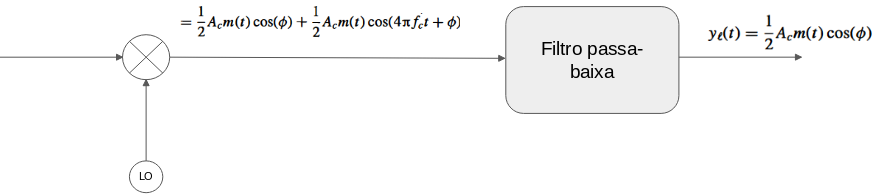
\includegraphics[width = 0.85\textwidth ]{Fig/rx_dsb.png}
    \caption{Filtragem das altas frequências}
  \end{figure}

  \begin{block}{Comentários}
    \begin{itemize}
     \item Um filtro passa-baixa é um componente eletrônico que permite a passagem de sinais com frequências abaixo de um limite específico, chamado de frequência de corte, e atenua os sinais com frequências acima desse limite. 
     \item É usado para remover ruídos e interferências de alta frequência indesejadas que ainda possam estar presentes no sinal. Isso melhora a qualidade do som reproduzido pelos alto-falantes ou fones de ouvido.
    \end{itemize}
  
  \end{block}


\end{frame}

\begin{frame}
  \frametitle{Sinal Demodulado}

  \begin{figure}[h!]
    \begin{center}
      \begin{tikzpicture}
        \begin{axis}[
            width=0.5\textwidth, % Scale the plot to \linewidth
            grid = major, % Display a grid
            grid style={dashed,gray!30}, % Set the style
            xlabel= Tempo, % Set the labels
            ylabel= Amplitude,
            ymin=-1, ymax=1,
            x unit=\si{\second}, % Set the respective units
            y unit=\si{\volt},
            legend style={at={(1,1)},anchor=north west} % Put the legend below the plot
            %x tick label style={rotate=90,anchor=east} % Display labels sideways
          ]
          
          \addplot+ [no marks]
          table[x=Tempo,y=Mensagem,col sep=comma] {Fig/sinal_estimado.csv}; 

          \addplot+ [no marks,black]
          table[x=Tempo,y=Mensagem_Estimada,col sep=comma] {Fig/sinal_estimado.csv}; 


          \legend{Mensagem, Mensagem estimada}
        \end{axis}
      \end{tikzpicture}
      \caption{Comparação entre a mensagem estimada e mensagem real.}
    \end{center}
  \end{figure}

\end{frame}


\section{AM Convencional}

\begin{frame}{Princípios da AM Convencional}
  
  \begin{itemize}
      \item Na AM convencional, a onda portadora e as duas bandas laterais (superior e inferior) são transmitidas.
      \item As bandas laterais são simétricas em relação à frequência da portadora e contêm a mesma informação.
      \item A largura de banda total de um sinal AM convencional é o dobro da largura de banda do sinal de informação.
  \end{itemize}
\end{frame}
 
\begin{frame}
  \begin{block}{Vantagens}
  \begin{itemize}
      \item Simplicidade: A modulação e a demodulação AM são relativamente simples de implementar.
      \item Compatibilidade: A AM convencional é compatível com a maioria dos rádios de ondas médias e curtas disponíveis no mercado.
  \end{itemize}
  \end{block}
  
  \begin{block}{Desvantagens}
  \begin{itemize}
      \item Largura de banda: A AM convencional é ineficiente em termos de largura de banda, pois transmite duas bandas laterais idênticas.
      \item Suscetibilidade a ruído: A AM convencional é mais suscetível a ruído e interferências, resultando em uma qualidade de áudio inferior em comparação com outras técnicas, como a modulação em frequência (FM) ou a modulação de banda lateral única (SSB).
      \item Eficiência energética: A AM convencional consome mais energia durante a transmissão, pois a onda portadora também é transmitida junto com as bandas laterais.
  \end{itemize}
  \end{block}

\end{frame}

\begin{frame}
  \frametitle{Sinal Modulado}

  \begin{columns}[T] % A opção "T" alinha o conteúdo das colunas pelo topo
    \begin{column}{0.5\textwidth}
      \begin{figure}[h!]
        \begin{center}
          \begin{tikzpicture}
            \begin{axis}[
                width=0.85\textwidth, % Scale the plot to \linewidth
                grid = major, % Display a grid
                grid style={dashed,gray!30}, % Set the style
                xlabel= Tempo, % Set the labels
                ylabel= Amplitude,
                ymin=-1.5, ymax=1.5,
                x unit=\si{\second}, % Set the respective units
                y unit=\si{\volt},
                legend style={at={(0,1.5)},anchor=north west} % Put the legend below the plot
                %x tick label style={rotate=90,anchor=east} % Display labels sideways
              ]
              
              \addplot+ [no marks]
              table[x=Tempo,y=Sinal,col sep=comma] {Fig/sinal_am_convencional.csv}; 
    
              \addplot+ [no marks,dashed,red]
              table[x=Tempo,y=Mensagem,col sep=comma] {Fig/sinal_am_convencional.csv}; 
    
    
              \legend{Sinal AM Convencional, Mensagem}
            \end{axis}
          \end{tikzpicture}
          \caption{Sinal AM convecional}
        \end{center}
      \end{figure}
    \end{column}
    \begin{column}{0.5\textwidth}
      \begin{block}{Equação}
        $$
        s(t)  = A_c \left(1 + \alpha m(t)\right) \cos(2\pi f_c t)
        $$
        \begin{itemize}
          \item $\alpha$ é índice de Modulação
          \item Sinal esta no envelope do sinal 
          \item Enviou de uma portadora adicional
        \end{itemize}
      \end{block}  

    \end{column}
\end{columns}

\end{frame}


\begin{frame}
  \frametitle{Sinal Modulado}

  \begin{columns}[T] % A opção "T" alinha o conteúdo das colunas pelo topo
    \begin{column}{0.5\textwidth}
      \begin{figure}[h!]
        \begin{center}
          \begin{tikzpicture}
            \begin{axis}[
                width=0.85\textwidth, % Scale the plot to \linewidth
                grid = major, % Display a grid
                grid style={dashed,gray!30}, % Set the style
                xlabel= Tempo, % Set the labels
                ylabel= Amplitude,
                ymin=-1.5, ymax=1.5,
                x unit=\si{\second}, % Set the respective units
                y unit=\si{\volt},
                legend style={at={(0,1.5)},anchor=north west} % Put the legend below the plot
                %x tick label style={rotate=90,anchor=east} % Display labels sideways
              ]
              
              \addplot+ [no marks]
              table[x=Tempo,y=Sinal,col sep=comma] {Fig/sinal_am_convencional.csv}; 
    
              \addplot+ [no marks,dashed,red]
              table[x=Tempo,y=Mensagem,col sep=comma] {Fig/sinal_am_convencional.csv}; 
    
    
              \legend{Sinal AM Convencional, Mensagem}
            \end{axis}
          \end{tikzpicture}
          \caption{Sinal AM convecional}
        \end{center}
      \end{figure}
    \end{column}
    \begin{column}{0.5\textwidth}
 
      \begin{figure}[h!]
        \begin{center}
          \begin{tikzpicture}
            \begin{axis}[
                width=0.85\textwidth, % Scale the plot to \linewidth
                grid = major, % Display a grid
                grid style={dashed,gray!30}, % Set the style
                xlabel= Frequência, % Set the labels
                ylabel= Amplitude,
                ymin=0, ymax=0.5,
                xmin = -200, xmax = 200,
                x unit=\si{\hertz}, % Set the respective units
                y unit=\si{\volt},
                legend style={at={(0,1.5)},anchor=north west}, % Put the legend below the plot
                %x tick label style={rotate=90,anchor=east} % Display labels sideways
              ]
              
            
              \addplot+ [no marks]
              table[x=Frequencia,y=Amplitude(V),col sep=comma] {Fig/sinal_freq_am_convencional.csv}; 
    
    
              \legend{Sinal Modulado}
            \end{axis}
          \end{tikzpicture}
          \caption{Representação em Frequencia do Sinal AM convencional.}
        \end{center}
      \end{figure}

    \end{column}
\end{columns}

\end{frame}

\begin{frame}
  \frametitle{Sinal de Demodulado: Retificação}

  \begin{columns}[T] % A opção "T" alinha o conteúdo das colunas pelo topo
    \begin{column}{0.5\textwidth}
      \begin{figure}[h!]
        \begin{center}
          \begin{tikzpicture}
            \begin{axis}[
                width=0.85\textwidth, % Scale the plot to \linewidth
                grid = major, % Display a grid
                grid style={dashed,gray!30}, % Set the style
                xlabel= Tempo, % Set the labels
                ylabel= Amplitude,
                ymin=0, ymax=1.5,
                x unit=\si{\second}, % Set the respective units
                y unit=\si{\volt},
                legend style={at={(0,1.5)},anchor=north west} % Put the legend below the plot
                %x tick label style={rotate=90,anchor=east} % Display labels sideways
              ]
              
              \addplot+ [no marks]
              table[x=Tempo,y=Sinal_retificado,col sep=comma] {Fig/sinal_am_convencional.csv}; 
    
              \addplot+ [no marks,dashed,red]
              table[x=Tempo,y=Mensagem,col sep=comma] {Fig/sinal_am_convencional.csv}; 
    
    
              \legend{Sinal retificado, Mensagem}
            \end{axis}
          \end{tikzpicture}
          \caption{Sinal AM convecional}
        \end{center}
      \end{figure}
    \end{column}
    \begin{column}{0.5\textwidth}
 
      \begin{figure}[h!]
        \begin{center}
          \begin{tikzpicture}
            \begin{axis}[
                width=0.85\textwidth, % Scale the plot to \linewidth
                grid = major, % Display a grid
                grid style={dashed,gray!30}, % Set the style
                xlabel= Frequência, % Set the labels
                ylabel= Amplitude,
                ymin=0, ymax=0.5,
                xmin = -400, xmax = 400,
                x unit=\si{\hertz}, % Set the respective units
                y unit=\si{\volt},
                legend style={at={(0,1.5)},anchor=north west}, % Put the legend below the plot
                %x tick label style={rotate=90,anchor=east} % Display labels sideways
              ]
              
            
              \addplot+ [no marks]
              table[x=Frequencia,y=Amplitude(V)2,col sep=comma] {Fig/sinal_freq_am_convencional.csv}; 
    
    
              \legend{Sinal Retificado}
            \end{axis}
          \end{tikzpicture}
          \caption{Representação em Frequencia do Sinal Retificado.}
        \end{center}
      \end{figure}

    \end{column}
\end{columns}

\end{frame}

\begin{frame}
  \frametitle{Sinal Demodulado: Filtragem}

  \begin{figure}[h!]
    \begin{center}
      \begin{tikzpicture}
        \begin{axis}[
            width=0.65\textwidth, % Scale the plot to \linewidth
            grid = major, % Display a grid
            grid style={dashed,gray!30}, % Set the style
            xlabel= Tempo, % Set the labels
            ylabel= Amplitude,
            ymin=-1.5, ymax=1.5,
            x unit=\si{\second}, % Set the respective units
            y unit=\si{\volt},
            legend style={at={(0,1)},anchor=north west} % Put the legend below the plot
            %x tick label style={rotate=90,anchor=east} % Display labels sideways
          ]
          
          \addplot+ [no marks]
          table[x=Tempo,y=Mensagem2,col sep=comma] {Fig/sinal_am_convencional.csv}; 

          \addplot+ [no marks,dashed,red]
          table[x=Tempo,y=Mensagem_estimada,col sep=comma] {Fig/sinal_am_convencional.csv}; 


          \legend{Mensagem, Mensagem Estimada} 
        \end{axis}
      \end{tikzpicture}
      \caption{Sinal demodulado}
    \end{center}
  \end{figure}

\end{frame}
\end{document}